\thispagestyle{timhieukhoahocnone}
\pagestyle{timhieukhoahoc}
\everymath{\color{timhieukhoahoc}}
\blfootnote{$^1$\text{\color{timhieukhoahoc}Hà Nội.}}
\graphicspath{{../timhieukhoahoc/pic2/}}
\begingroup
\AddToShipoutPicture*{\put(0,616){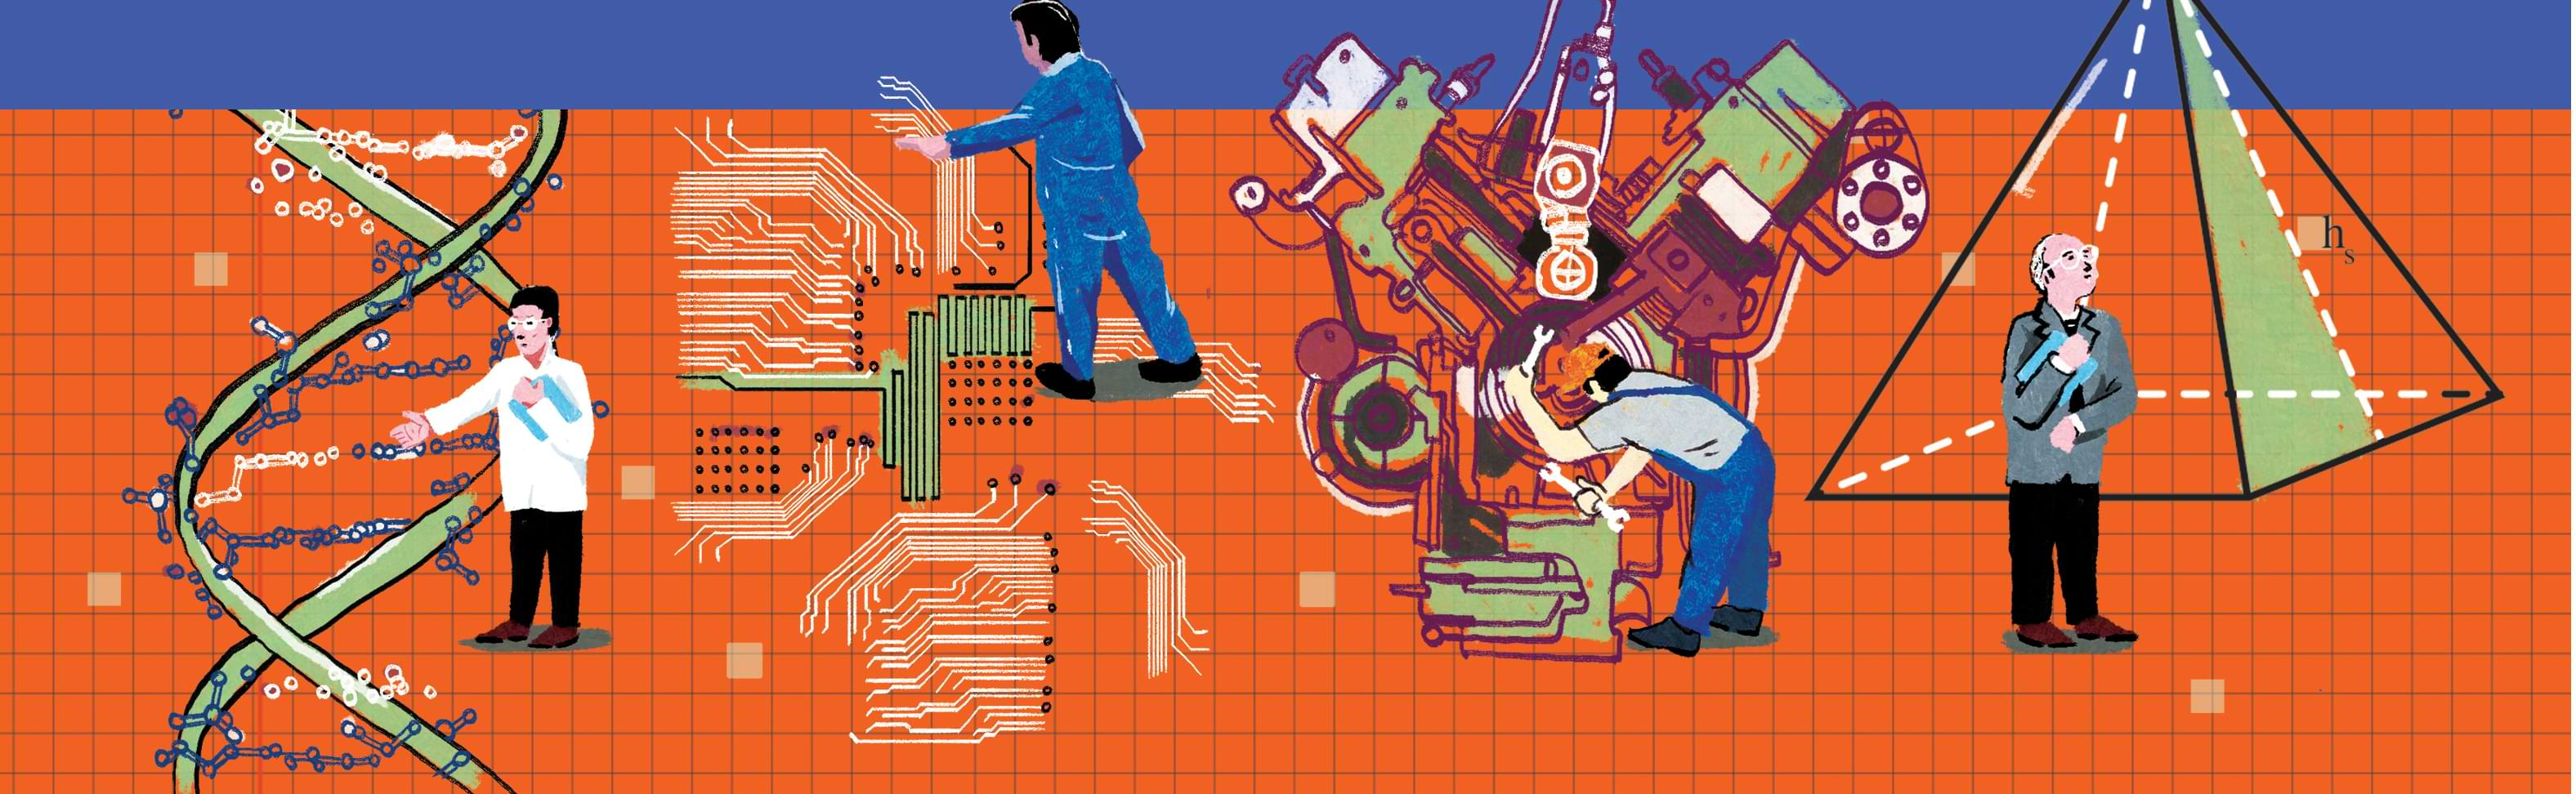
\includegraphics[width=19.3cm]{../bannertimhieu}}}
\AddToShipoutPicture*{\put(41,552){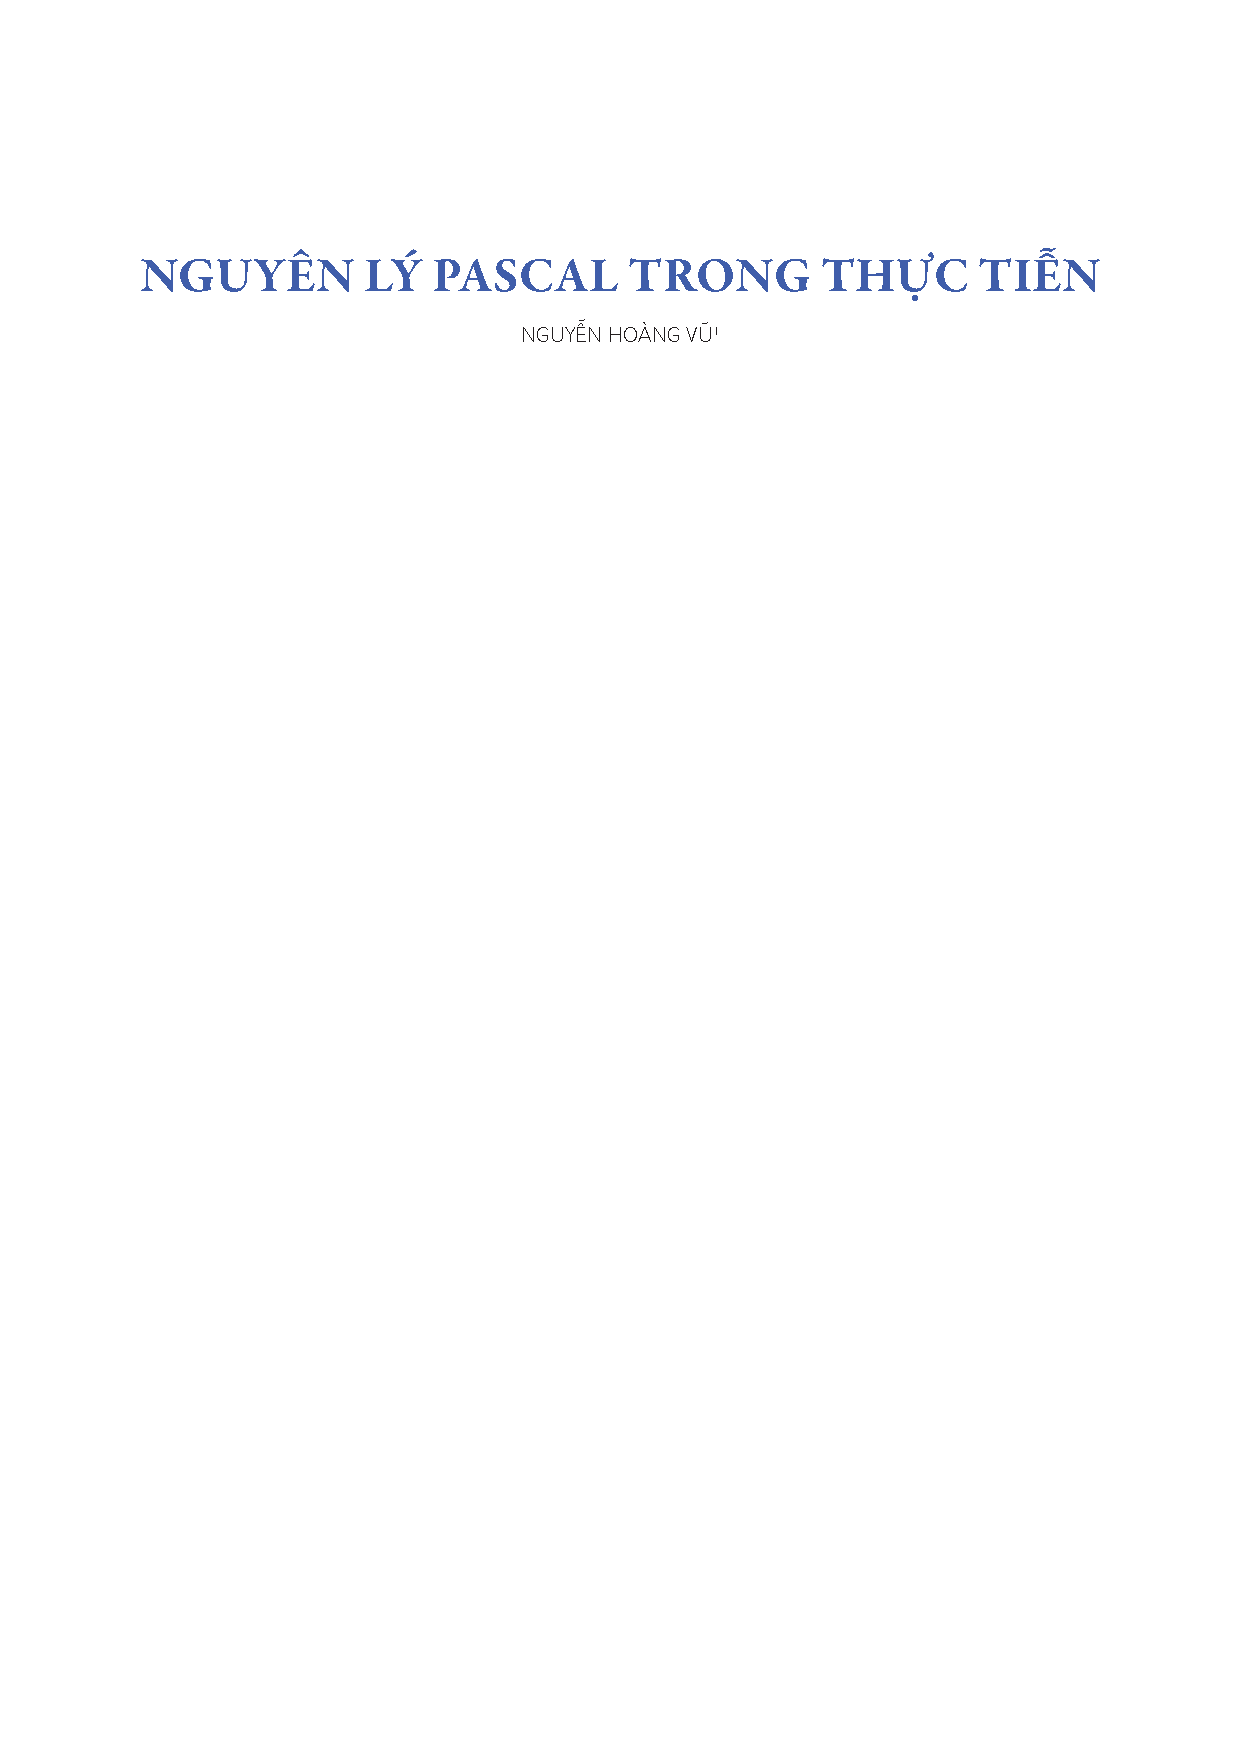
\includegraphics[scale=1]{../tieude1.pdf}}}
\centering
\endgroup
\vspace*{155pt}

\begin{multicols}{2}
	Trong số trước của Pi, chúng ta đã tìm hiểu quá trình Pascal khám phá ra nguyên lý mang tên ông về áp suất trong lòng chất lỏng. Bài viết này sẽ trình bày những ứng dụng của nguyên lý trên trong các hiện tượng tự nhiên cũng như các công cụ sử dụng thủy lực đa dạng trong đời sống.
	\vskip 0.1cm
	$\pmb{1.}$ \textbf{\color{timhieukhoahoc}Ứng dụng của bình thông nhau}
	\begin{figure}[H]
		\vspace*{-5pt}
		\centering
		\captionsetup{labelformat= empty, justification=centering}
		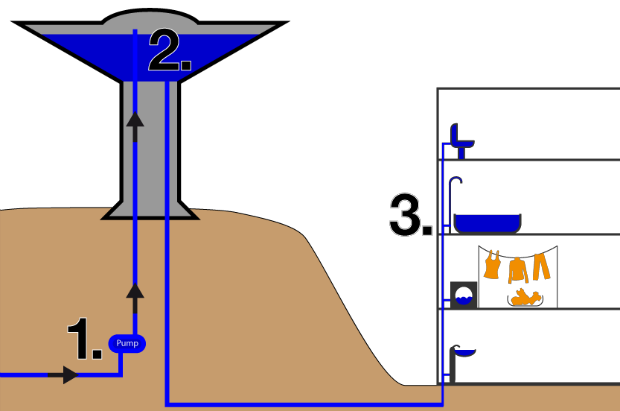
\includegraphics[width= 1\linewidth]{1}
		\caption{\small\textit{\color{timhieukhoahoc}Hình $1$. Quy trình hoạt động của tháp nước: $1$. Nước được bơm lên bể trên tháp. $2$. Bể trên tháp có tác dụng như cột nước ở một nhánh của bình thông nhau. $3$. Các vòi nước ở nhà dân đóng vai trò nhánh còn lại.}}
		\vspace*{-5pt}
	\end{figure}
	Một ứng dụng rất thực tế của mô hình bình thông nhau trong đời sống là các tháp nước. Nước được bơm lên và chứa trong các bể cao ở đỉnh tháp. Áp suất do nước trong bể sẽ được truyền theo đường ống và tạo thành áp suất nước khi ta mở các van lấy nước sinh hoạt. Với những tầng nhà càng cao thì áp suất nước sẽ càng giảm đi do chênh lệch độ cao với tháp nước giảm. Các đài phun nước cũng là một ứng dụng khác của bình thông nhau trong thực tiễn đời sống.
	Một hiện tượng tương tự trong tự nhiên là các giếng phun. Ở những vị trí có độ cao nằm dưới mực nước ngầm của một khu vực, khi ta khoan giếng, việc này cũng giống như mở một nhánh mới của bình thông nhau và áp suất nước sẽ khiến nước tự phun lên mặt đất giống như vòi phun vậy. 
	\begin{figure}[H]
		\vspace*{-5pt}
		\centering
		\captionsetup{labelformat= empty, justification=centering}
		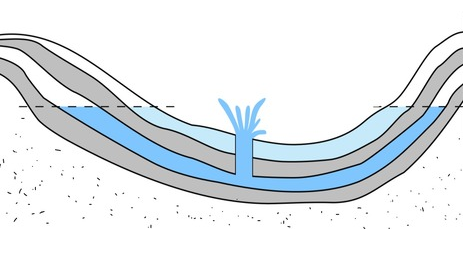
\includegraphics[width= 1\linewidth]{2}
		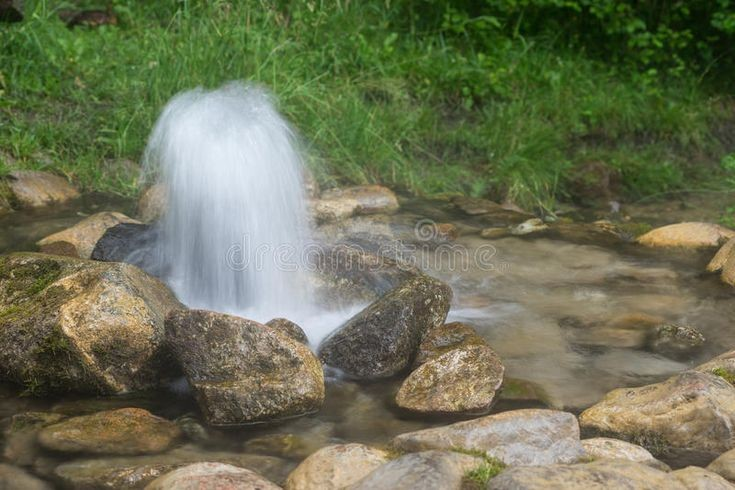
\includegraphics[width= 1\linewidth]{3}
		\caption{\small\textit{\color{timhieukhoahoc}Hình $2$. Giếng phun trong tự nhiên xuất hiện tại các vị trí nằm dưới mực nước ngầm của khu vực.}}
		\vspace*{-5pt}
	\end{figure}
	\begin{figure}[H]
		\vspace*{5pt}
		\centering
		\captionsetup{labelformat= empty, justification=centering}
		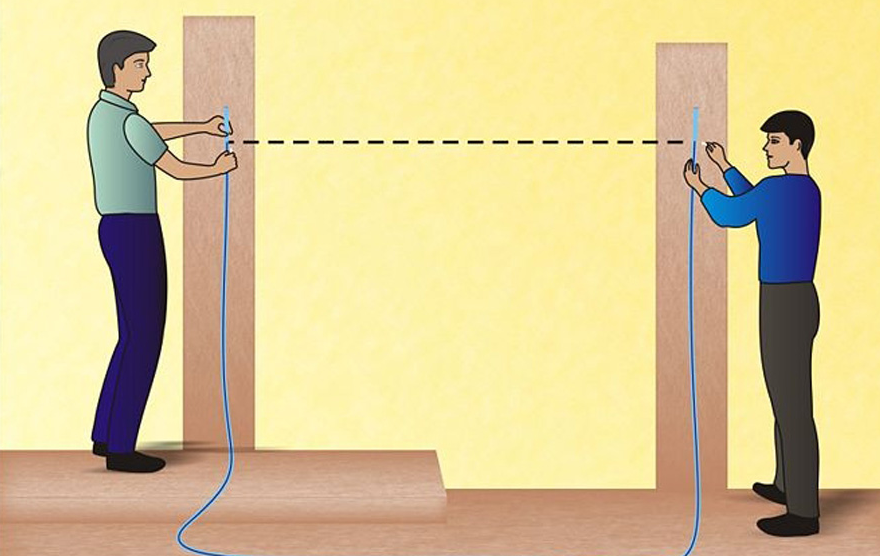
\includegraphics[width= 1\linewidth]{4}
		\caption{\small\textit{\color{timhieukhoahoc}Hình $3$. Gióng hàng theo phương ngang sử dụng ống chứa nước. Đây là một phương pháp rẻ và hiệu quả trước khi có sự xuất hiện của các thiết bị sử dụng laser.}}
		\vspace*{-10pt}
	\end{figure}
	Do mực nước ở hai nhánh của bình thông nhau luôn ngang hàng nên trong xây dựng, người ta có thể dùng một ống nhựa trong suốt (hoặc hai hình trụ thủy tinh gắn với hai đầu một ống nối) chứa nước để tiến hành gióng hàng theo phương ngang. Thao tác gióng hàng sẽ cần có hai người. Một người giữ một nhánh ống ở vị trí cố định. Người kia dùng mực nước ở nhánh còn lại để đánh dấu vị trí ngang hàng. Các bạn học sinh cũng có thể thử làm thí nghiệm này trên lớp nhưng cần chú ý không bao giờ để hai đầu ống có chênh lệch độ cao quá lớn, nếu không nước sẽ bị trào ra. 
	\begin{figure}[H]
		\vspace*{-5pt}
		\centering
		\captionsetup{labelformat= empty, justification=centering}
		
\includegraphics[width= 1\linewidth]{5}
		\caption{\small\textit{\color{timhieukhoahoc}Hình $4$. Khi đo huyết áp, vị trí đo cần ngang hàng với tim để kết quả đo được chính xác.}}
		\vspace*{-10pt}
	\end{figure}
	Tương tự, khi bác sĩ tiến hành đo huyết áp cho bệnh nhân, để kết quả đo gần với áp suất của máu ở tim nhất, vị trí đo huyết áp cần có độ cao ngang hàng với tim của người được đo. Thật vậy, hệ tuần hoàn của cơ thể cũng giống như một hệ thống bình thông nhau với nhiều nhánh!
	\vskip 0.1cm
	Cơ chế hoạt động trên cũng có thể được sử dụng để chế tạo thiết bị đo áp suất. Nếu ta đổ chất lỏng vào một bình thông nhau dạng chữ U, khi cả hai đầu của mỗi nhánh đều hở và tiếp xúc với không khí thì mực chất lỏng ở hai nhánh sẽ bằng nhau. Nếu một đầu được cho tiếp xúc với một bình chứa khí thì độ chênh lệch mực chất lỏng giữa hai nhánh sẽ cho ta độ chênh lệch về áp suất của khí trong bình chứa với áp suất khí quyển:
	\begin{align*}
		\Delta p = \rho g |\Delta h|
	\end{align*}
	với $\rho$ là mật độ của chất lỏng trong ống. 
	\vskip 0.1cm
	Nếu mực chất lỏng trong nhánh tiếp xúc với bình chứa khí thấp hơn nhánh còn lại thì áp suất trong bình chứa sẽ cao hơn áp suất khí quyển. Ngược lại, nếu mực chất lỏng trong ống này thấp hơn nhánh tiếp xúc với không khí thì áp suất của khối khí sẽ thấp hơn áp suất của khí quyển.
	\vskip 0.1cm
	Tương tự, nếu mỗi nhánh của ống tiếp xúc với một khối khí khác nhau, ta cũng có thể dùng cách này để đo sự chênh lệch áp suất giữa hai khối khí đó giống với trường hợp so sánh với áp suất khí quyển (Hình $5b$). Cách làm này có thể giúp xác định rò rỉ của đường ống dẫn khí bằng cách đo chênh lệch áp suất giữa hai vị trí khác nhau của đường ống.
	\vskip 0.1cm
	Người ta cũng có thể đo giá trị tuyệt đối của áp suất thay cho độ chênh lệch áp suất nếu một nhánh của ống là kín và phần phía trên của mặt chất lỏng là chân không. Trong trường hợp độ cao của cột chất lỏng quá lớn, ta có thể lắp nhiều ống chữ U nối với nhau, phần giữa của chúng được bơm khí nén có tác dụng truyền áp suất giống như với chất lỏng (Hình $5d$). Để tìm giá trị đo của áp suất, ta cần lấy tổng tất cả các độ chênh lệch mực chất lỏng của các ống chữ U.
	\begin{figure}[H]
		\vspace*{5pt}
		\centering
		\captionsetup{labelformat= empty, justification=centering}
		$a)$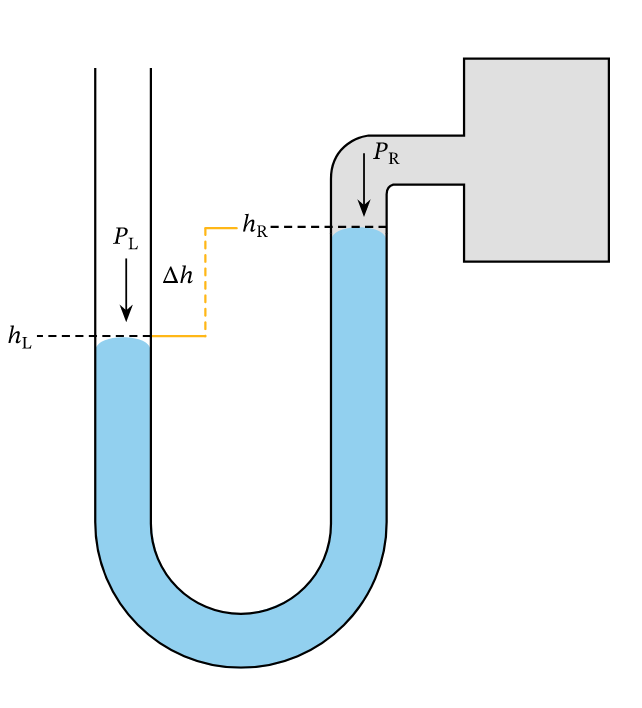
\includegraphics[height = 0.4\linewidth]{6}
		$b)$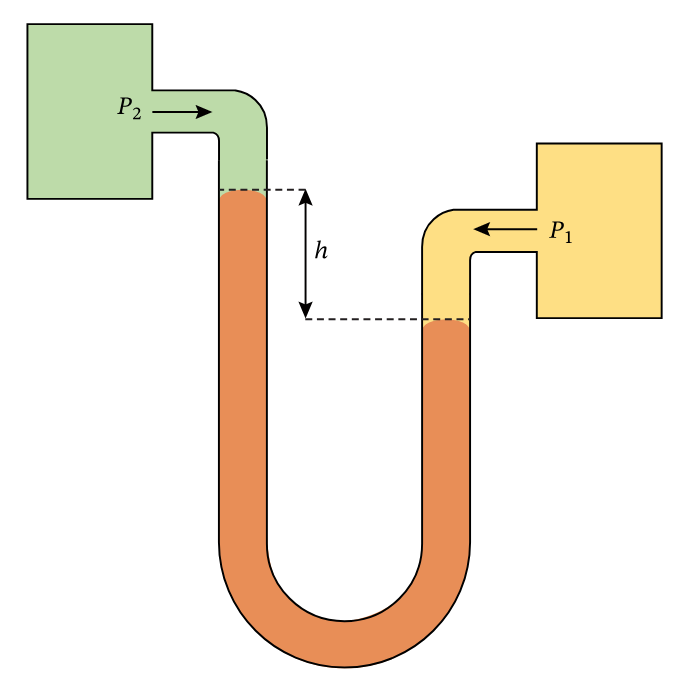
\includegraphics[height = 0.4\linewidth]{7}
		
		$c)$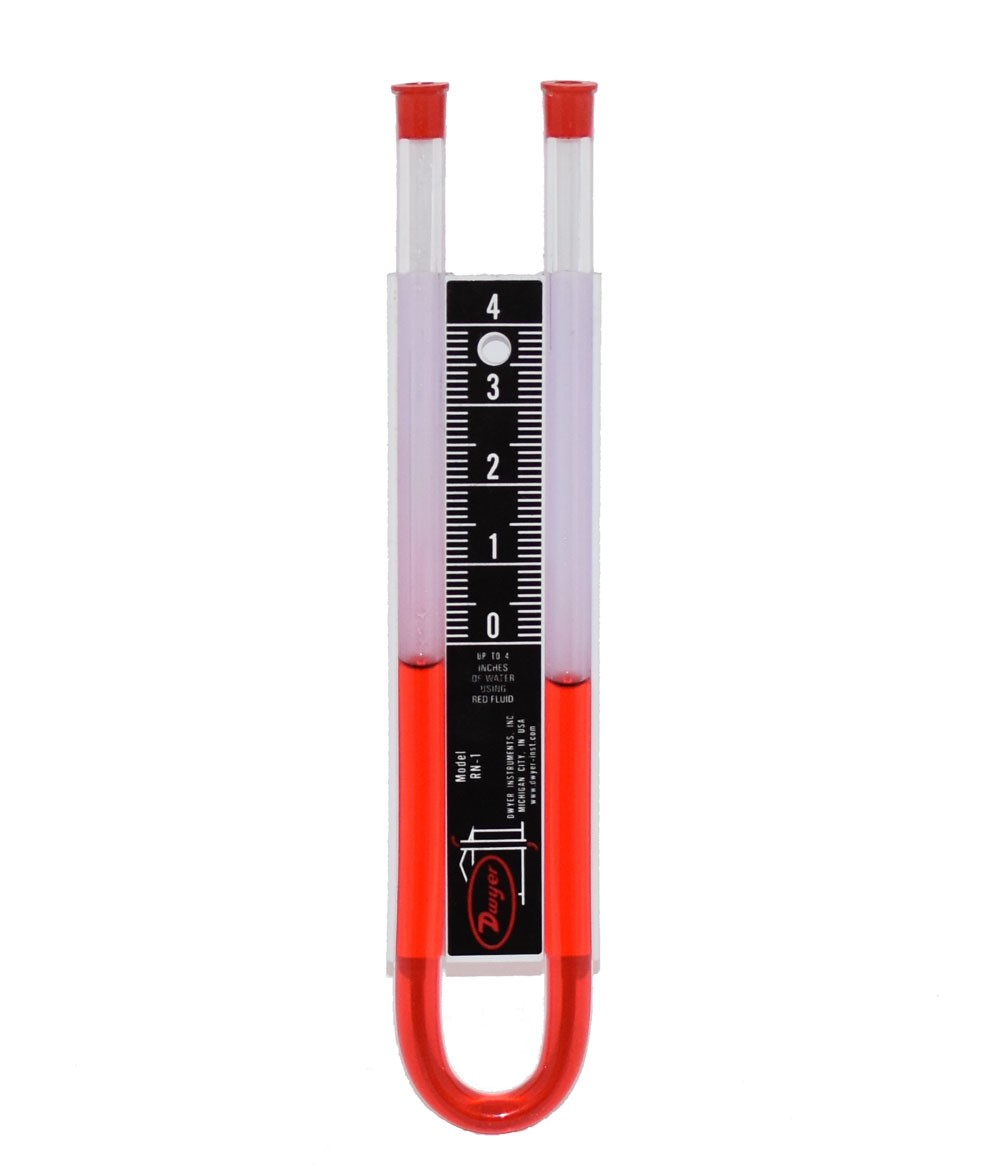
\includegraphics[height = 0.4\linewidth]{8}
		$d)$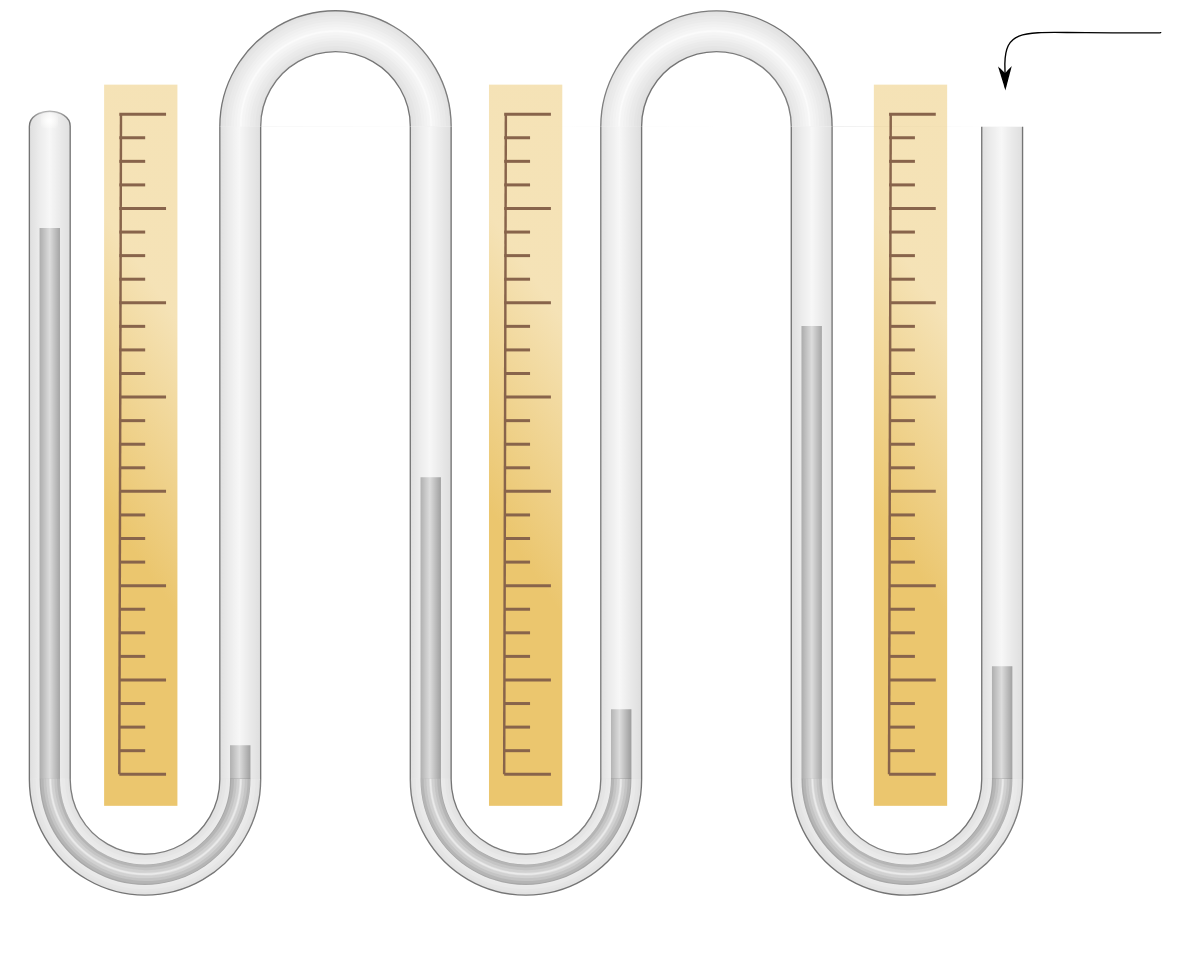
\includegraphics[height = 0.4\linewidth]{9}
		\caption{\small\textit{\color{timhieukhoahoc}Hình $5$. Đo áp suất chất khí bằng ống chữ U. $a)$ Đo chênh lệch áp suất của khối khí so với khí quyển. $b)$ Đo chênh lệch áp suất giữa hai chất khí. $c)$ Ống chữ U đo áp suất trong thực tế. $d)$ Nối các ông chữ U liên tiếp với nhau cho phép đo các áp suất lớn.}}
		\vspace*{-10pt}
	\end{figure}
	Một dạng biến thể khác của ống chữ U được thiết kế với một nhánh có thiết diện lớn hơn nhiều nhánh còn lại (tạo thành một giếng). Khi tiến hành đo, áp suất lớn hơn bao giờ cũng được gắn vào nhánh có giếng. Độ chênh lệch chất lỏng giữa hai nhánh vẫn sẽ giống như với ống chữ U thông thường nhưng chất lỏng bên nhánh giếng sẽ bị dịch chuyển ít hơn nhiều. Người ta có thể tính toán bù trừ lại sự dịch chuyển này để thiết lập thang đo trực tiếp cho nhánh còn lại. Nhánh còn lại cũng có thể được thay bằng một nhánh nghiêng cho độ nhạy tốt hơn và giúp đo các chênh lệch áp suất nhỏ hơn.
	\begin{figure}[H]
		\vspace*{-5pt}
		\centering
		\captionsetup{labelformat= empty, justification=centering}
		$a)$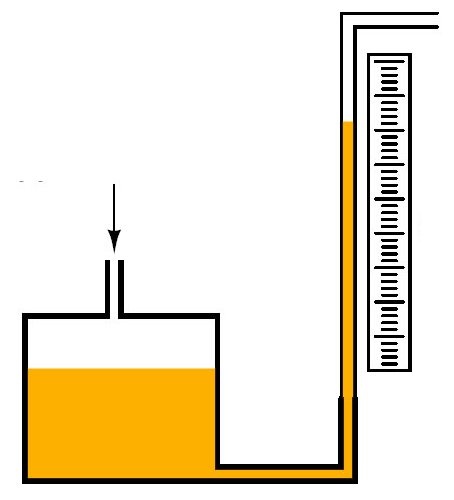
\includegraphics[height = 0.31\linewidth]{10}
		$b)$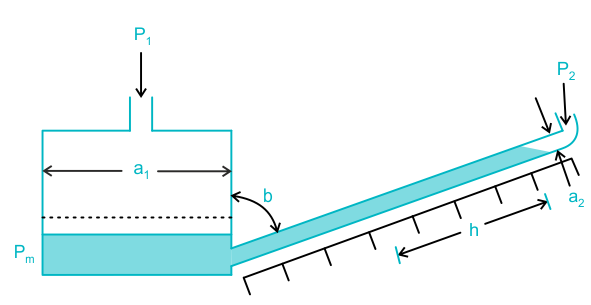
\includegraphics[height = 0.31\linewidth]{11}
		\caption{\small\textit{\color{timhieukhoahoc}Hình $6$. $a)$ Ống chữ U đo áp suất với một nhánh dạng giếng. $b)$ Một nhánh có dạng giếng, nhánh còn lại là nhánh nghiêng.}}
		\vspace*{-10pt}
	\end{figure}
	\textbf{\color{timhieukhoahoc}Bài tập}
	\vskip 0.1cm
	$1$. Trong hình $6a$, giếng có thiết diện $S_1$, nhánh còn lại có thiết diện $S_2$. Ban đầu hai mực chất lỏng sẽ ngang nhau. Khi có chênh lệch áp suất ứng với chênh lệch độ cao $\Delta h$ giữa hai mực chất lỏng, mực chất lỏng trong nhánh có giếng sẽ đi xuống một đoạn $h_1$ còn mực chất lỏng trong nhánh còn lại sẽ dâng lên một đoạn $h_2$.
	\vskip 0.1cm
	$a)$ Viết phương trình liên hệ $\Delta h,h_1,h_2$.
	\vskip 0.1cm
	$b)$ Viết phương trình liên hệ $h_1,h_2,S_1,S_2$.
	\vskip 0.1cm
	$c)$ Thiết lập biểu thức của $h_2$ theo $\Delta h$ và đề xuất cách tạo thang vạch chia để đọc $\Delta h$ theo mực chất lỏng bên nhánh nhỏ.
	\vskip 0.1cm
	$2.$ Làm tương tự bài $1$ cho trường hợp hình $6b$. Nhánh nghiêng tạo một góc $\alpha$ so với phương nằm ngang.
	\begin{figure}[H]
		\vspace*{-5pt}
		\centering
		\captionsetup{labelformat= empty, justification=centering}
		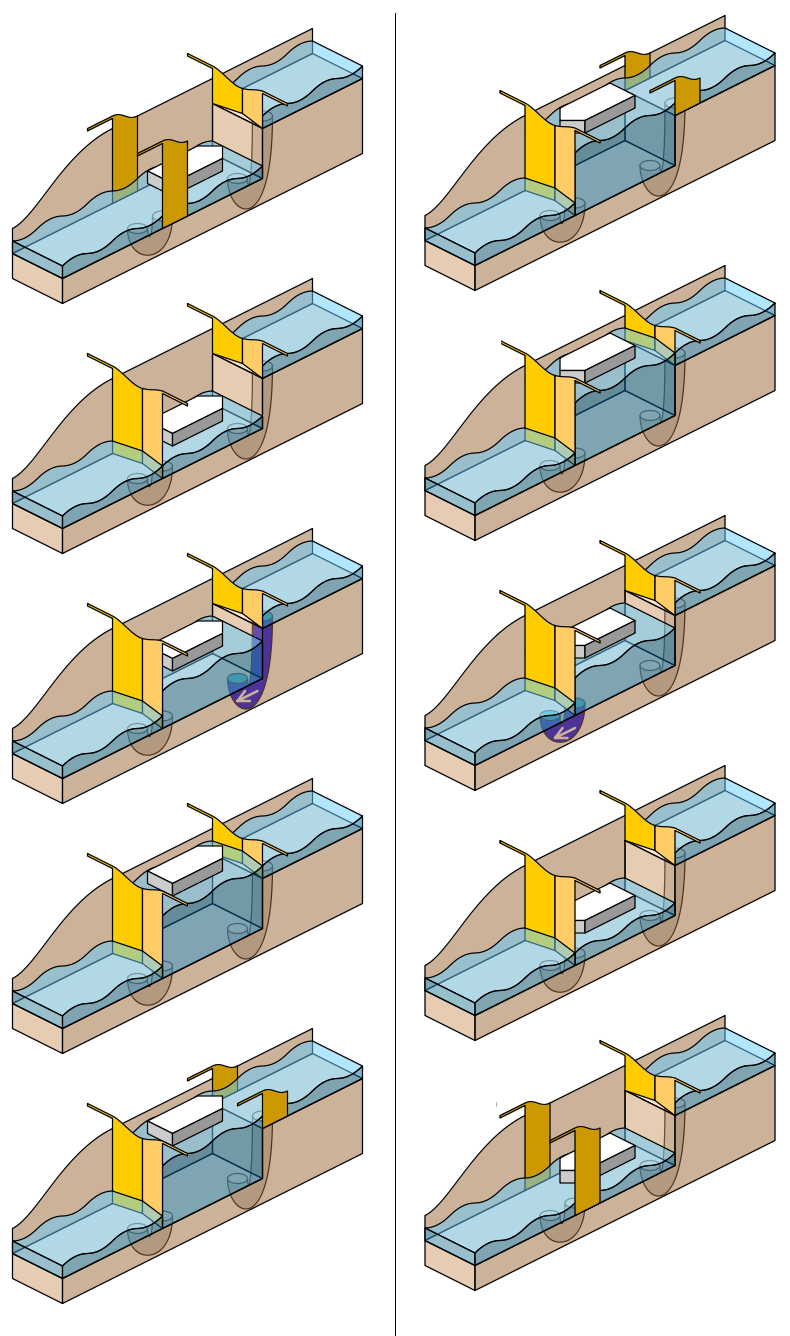
\includegraphics[width= 0.5\linewidth]{12}
		\caption{\small\textit{\color{timhieukhoahoc}Hình $6$. Di chuyển tàu giữa hai mực nước chênh lệch nhau ở hai phía đập. Trái: tàu đi lên cao. Phải: tàu đi xuống thấp.}}
		\vspace*{-10pt}
	\end{figure}
	Cơ chế của bình thông nhau còn xuất hiện trong các hệ thống vận chuyển tàu thuyền qua các con đập. Người ta tạo một khoảng trung gian giữa hai mực nước với hai cửa chặn. Khi tàu đi vào khoảng này, cả hai cửa đều được đóng. Sau đó người ta mở van ở phía tàu muốn tới. Theo nguyên tắc của bình thông nhau, sau một thời gian, mực nước ở vị trí tàu và phía nó muốn đến sẽ bằng nhau. Chỉ cần mở cửa ở phía này là tàu có thể tiếp tục đi được. Phương pháp trên có thể giúp tàu đi lên cao hoặc xuống thấp cho dù hai phía đập có chênh lệch về độ cao. Trong một số trường hợp, đề tăng hiệu quả sử dụng nước, các hệ thống vận chuyển này được thiết kế ở dạng nhiều tầng. 
	\vskip 0.1cm
	Hệ thống di chuyển tàu thuyền qua đập như trên lần đầu tiên được xây dựng ở Trung Quốc vào cuối thế kỷ $10$ thời nhà Tống. Các công trình tương tự chỉ bắt đầu xuất hiện ở châu Âu vào cuối thế kỷ $14$. Ngày nay, nhiều đập lớn hiện đại như kênh đào Panama sử dụng cách này để giúp tàu thuyền lưu thông qua đập. 
	\vskip 0.1cm
	$\pmb{2.}$ \textbf{\color{timhieukhoahoc}Khuyếch đại lực nhờ hệ thống thủy lực}
	\begin{figure}[H]
		\vspace*{-5pt}
		\centering
		\captionsetup{labelformat= empty, justification=centering}
		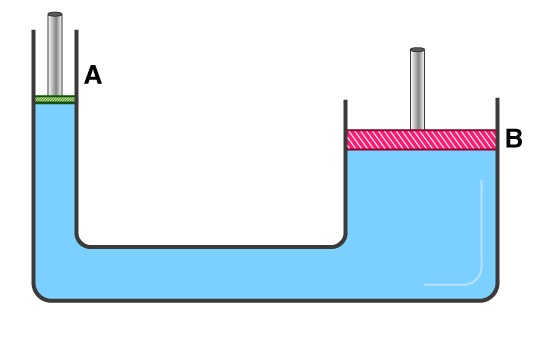
\includegraphics[width= 1\linewidth]{13}
		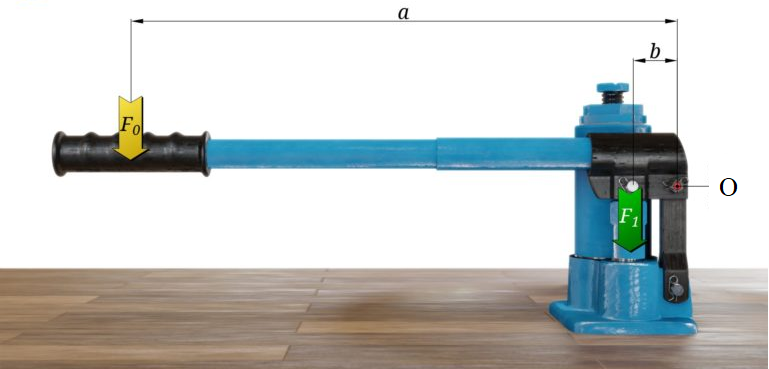
\includegraphics[width= 1\linewidth]{14}
		\caption{\small\textit{\color{timhieukhoahoc}Hình $7$. Cấu tạo của một kích thủy lực. Trên: hai piston ở hai nhánh của bình thông nhau. Dưới: đòn bẩy giúp tăng cường lực ép lên piston nhỏ. Lực ấn của tay được khuyếch đại theo tỉ lệ giữa hai tay đòn.}}
		\vspace*{-10pt}
	\end{figure}
	Việc khuyếch đại lực nhờ thủy lực cũng có nhiều ứng dụng trong đời sống. Một ví dụ thường được nhắc đến là kích thủy lực. Cấu tạo cơ bản của nó gồm hai piston ở hai nhánh của một bình thông nhau. Khi ta tác dụng một lực lên piston của nhánh nhỏ thì lực này được khuyếch đại ở piston của nhánh lớn. Trước đó, lực ấn của tay cũng đã được khuyếch đại một lần thông qua một đòn bẩy với độ khuyếch đại bằng với tỉ lệ tay đòn của vị trí ấn tay và vị trí của piston nhỏ. Hệ thống kích thủy lực dạng này giúp ta nâng lên những vật thể nặng, thậm chí cả các phương tiện như ô tô, tùy theo cấu tạo và khả năng khuyếch đại của kích thủy lực. Một số thiết bị sử dụng nguyên lý này được minh họa trong Hình $8$. Trong một số loại thang máy, hệ thống thủy lực cũng được sử dụng để di chuyển thang máy thay vì sử dụng một bộ ròng rọc.
	\begin{figure}[H]
		\vspace*{-5pt}
		\centering
		\captionsetup{labelformat= empty, justification=centering}
		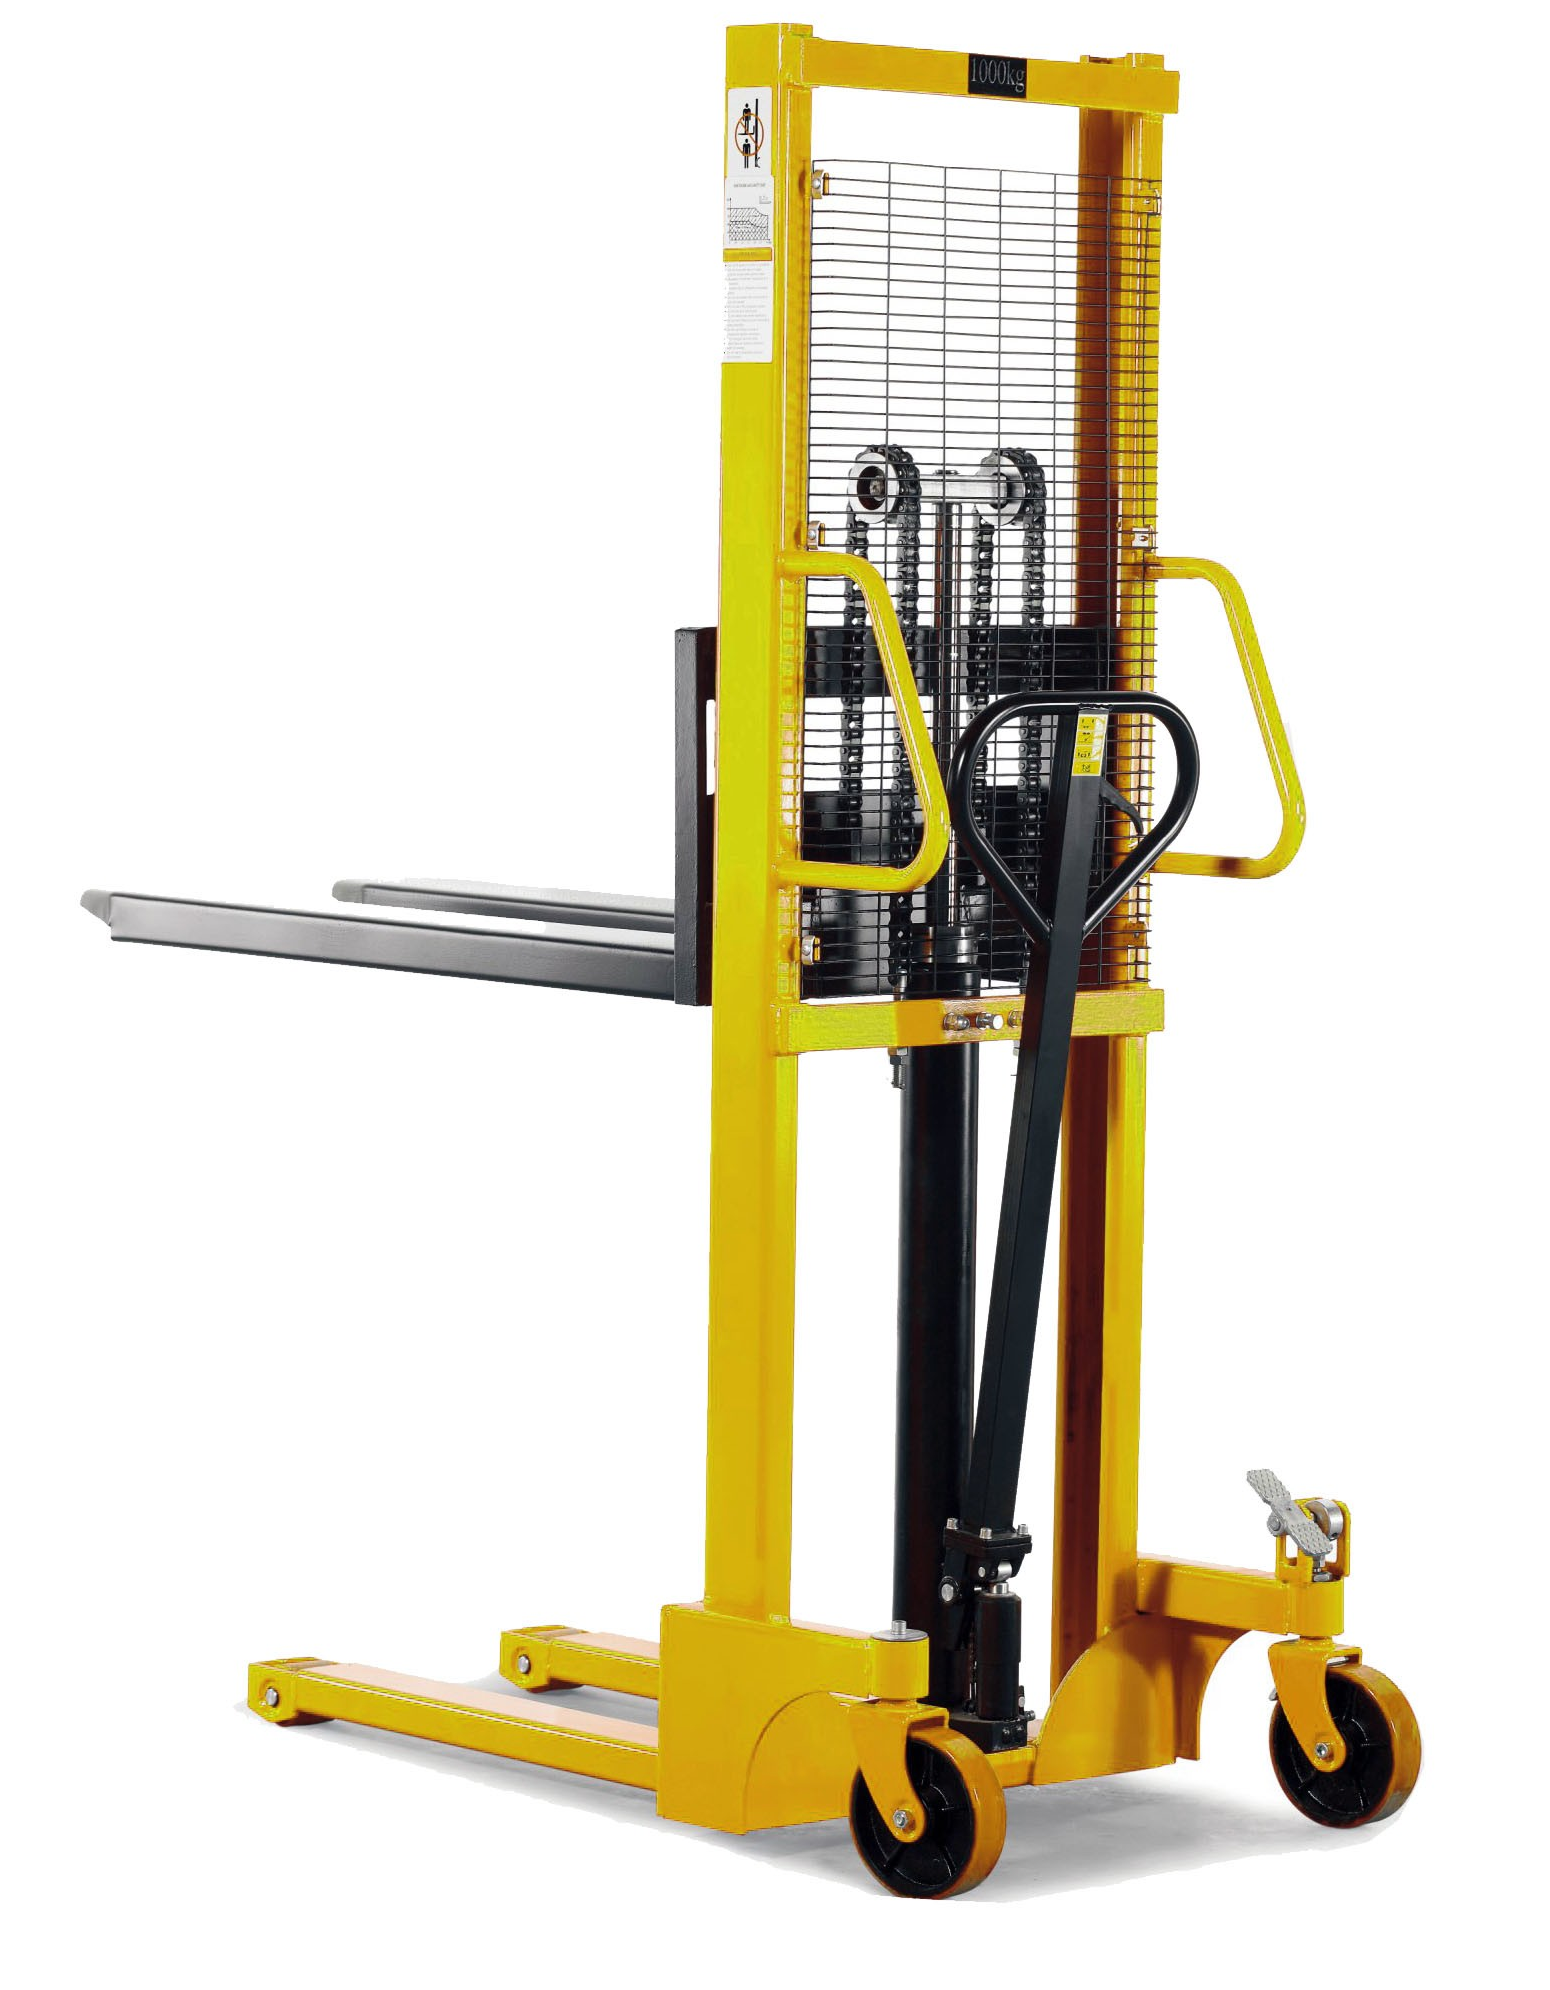
\includegraphics[height= 0.55\linewidth]{15}
		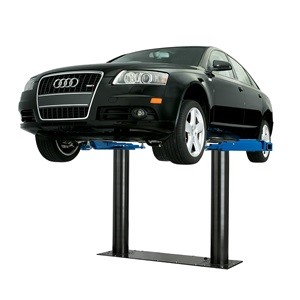
\includegraphics[height= 0.55\linewidth]{16}
		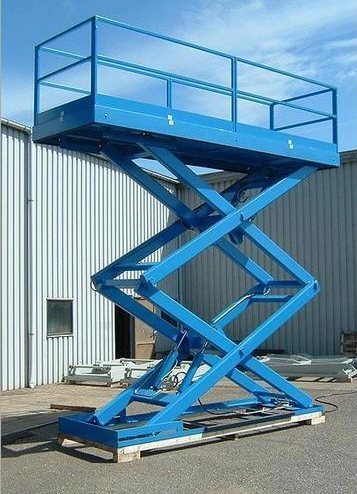
\includegraphics[height= 0.465\linewidth]{17}
		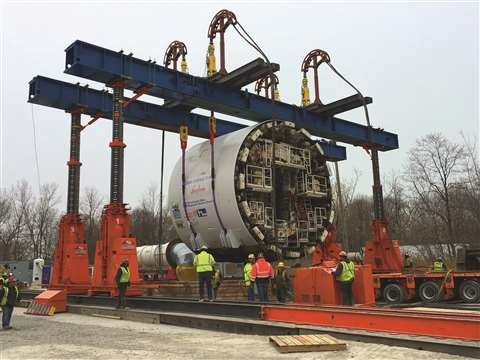
\includegraphics[height= 0.465\linewidth]{18}
		\caption{\small\textit{\color{timhieukhoahoc}Hình $8$. Một số thiết bị nâng sử dụng thủy lực trong sản xuất và vận chuyển.}}
		\vspace*{-10pt}
	\end{figure}
	Hệ thống nâng thủy lực cũng có thể được dùng ở một số cầu nơi có nhiều tàu thuyền đi lại. Vào những giờ cố định, nhịp cầu sẽ được kéo mở hoặc đẩy lên để các tàu thuyền với chiều cao lớn có thể đi qua bên dưới.
	\begin{figure}[H]
		\vspace*{-5pt}
		\centering
		\captionsetup{labelformat= empty, justification=centering}
		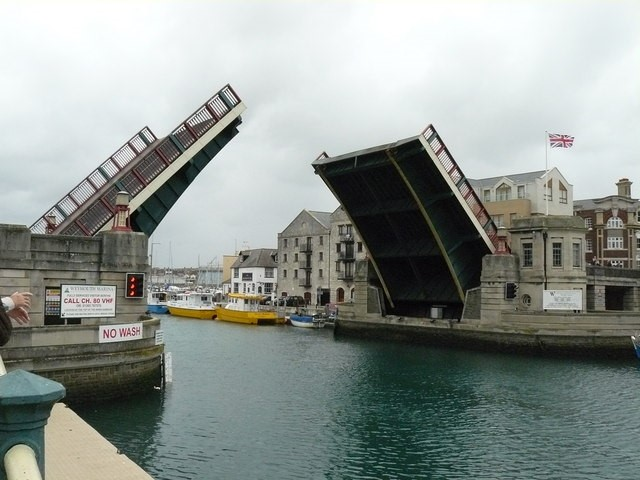
\includegraphics[width= 1\linewidth]{19}
		%		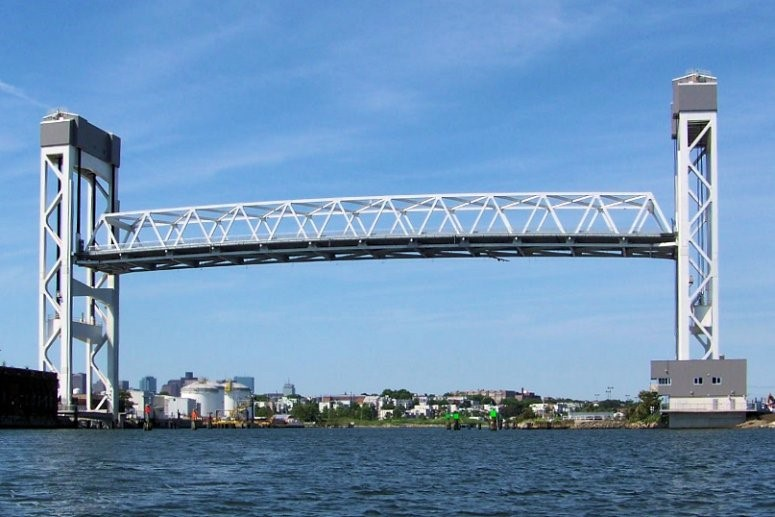
\includegraphics[width= 1\linewidth]{20}
		%		\caption{\small\textit{\color{timhieukhoahoc}Hình $9$. Một số cầu có hệ thống thủy lực để di chuyển nhịp cầu cho tàu thuyền đi qua.}}
		\vspace*{-10pt}
	\end{figure}
	\begin{figure}[H]
		\vspace*{5pt}
		\centering
		\captionsetup{labelformat= empty, justification=centering}
		%		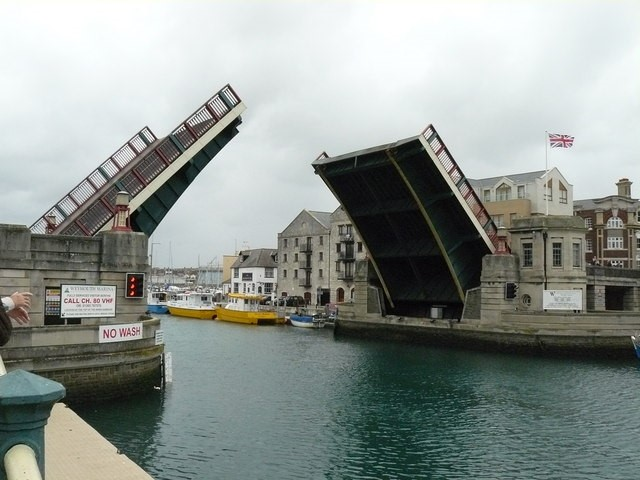
\includegraphics[width= 1\linewidth]{19}
		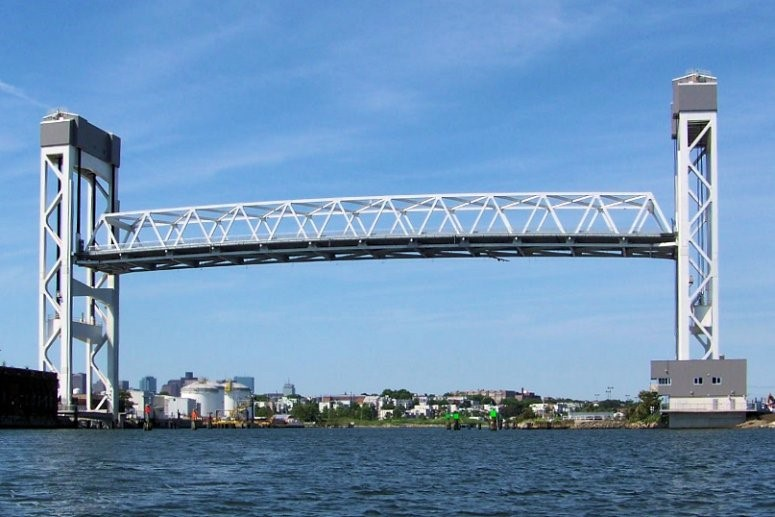
\includegraphics[width= 1\linewidth]{20}
		\caption{\small\textit{\color{timhieukhoahoc}Hình $9$. Một số cầu có hệ thống thủy lực để di chuyển nhịp cầu cho tàu thuyền đi qua.}}
		\vspace*{-10pt}
	\end{figure}
	Trong trường hợp piston lớn có chuyển động hướng xuống phía dưới, thay vì hệ thống nâng, ta có một hệ thống nén thủy lực. Hệ thống nén dạng này có nhiều ứng dụng trong công nghiệp như giúp nén phẳng các tấm kim loại, nghiền phế liệu, ...
	\begin{figure}[H]
		\vspace*{-5pt}
		\centering
		\captionsetup{labelformat= empty, justification=centering}
		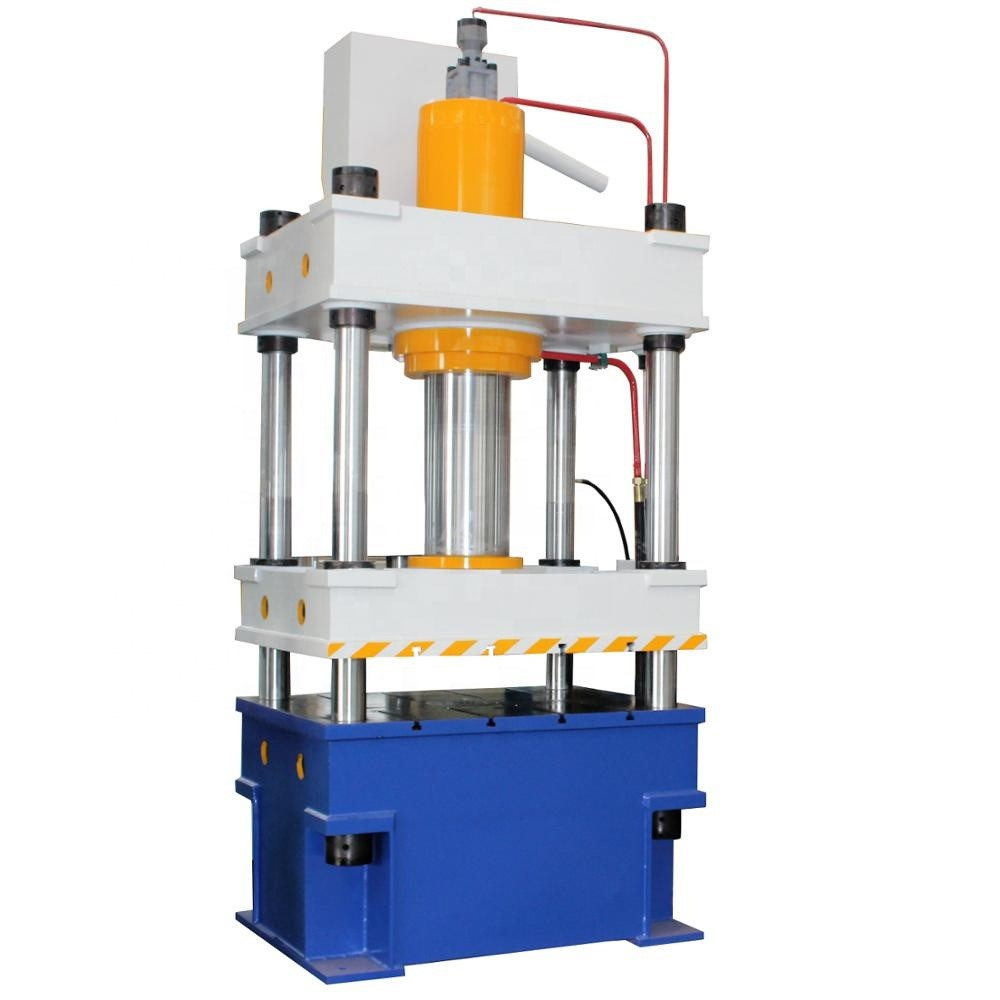
\includegraphics[width= 0.85\linewidth]{21}
		\caption{\small\textit{\color{timhieukhoahoc}Hình $10$. Máy ép thủy lực. Piston lớn sẽ chuyển động theo phương hướng xuống trong các thiết bị này.}}
		\vspace*{-10pt}
	\end{figure}
	Do đặc điểm truyền áp suất theo chất lỏng, hệ thống thủy lực trong công nghiệp không chỉ giúp khuếch đại lực mà còn có tác dụng làm chuyển hướng lực. Ví dụ như trong một máy xúc, cánh tay của nó cần phải gấp ở những khớp nối. Các đường ống dẫn chất lỏng (màu đen trong hình) có thể uốn cùng với chuyển động của cánh tay và cho phép truyền lực theo bất cứ hướng nào mà ta muốn.
	\begin{figure}[H]
		%		\vspace*{5pt}
		\centering
		\captionsetup{labelformat= empty, justification=centering}
		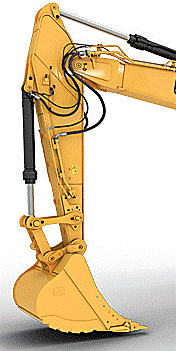
\includegraphics[width= 0.45\linewidth]{22}
		\caption{\small\textit{\color{timhieukhoahoc}Hình $11$. Tay máy xúc được điều khiển bằng thủy lực.}}
		\vspace*{-10pt}
	\end{figure}
	\begin{figure}[H]
		\vspace*{-5pt}
		\centering
		\captionsetup{labelformat= empty, justification=centering}
		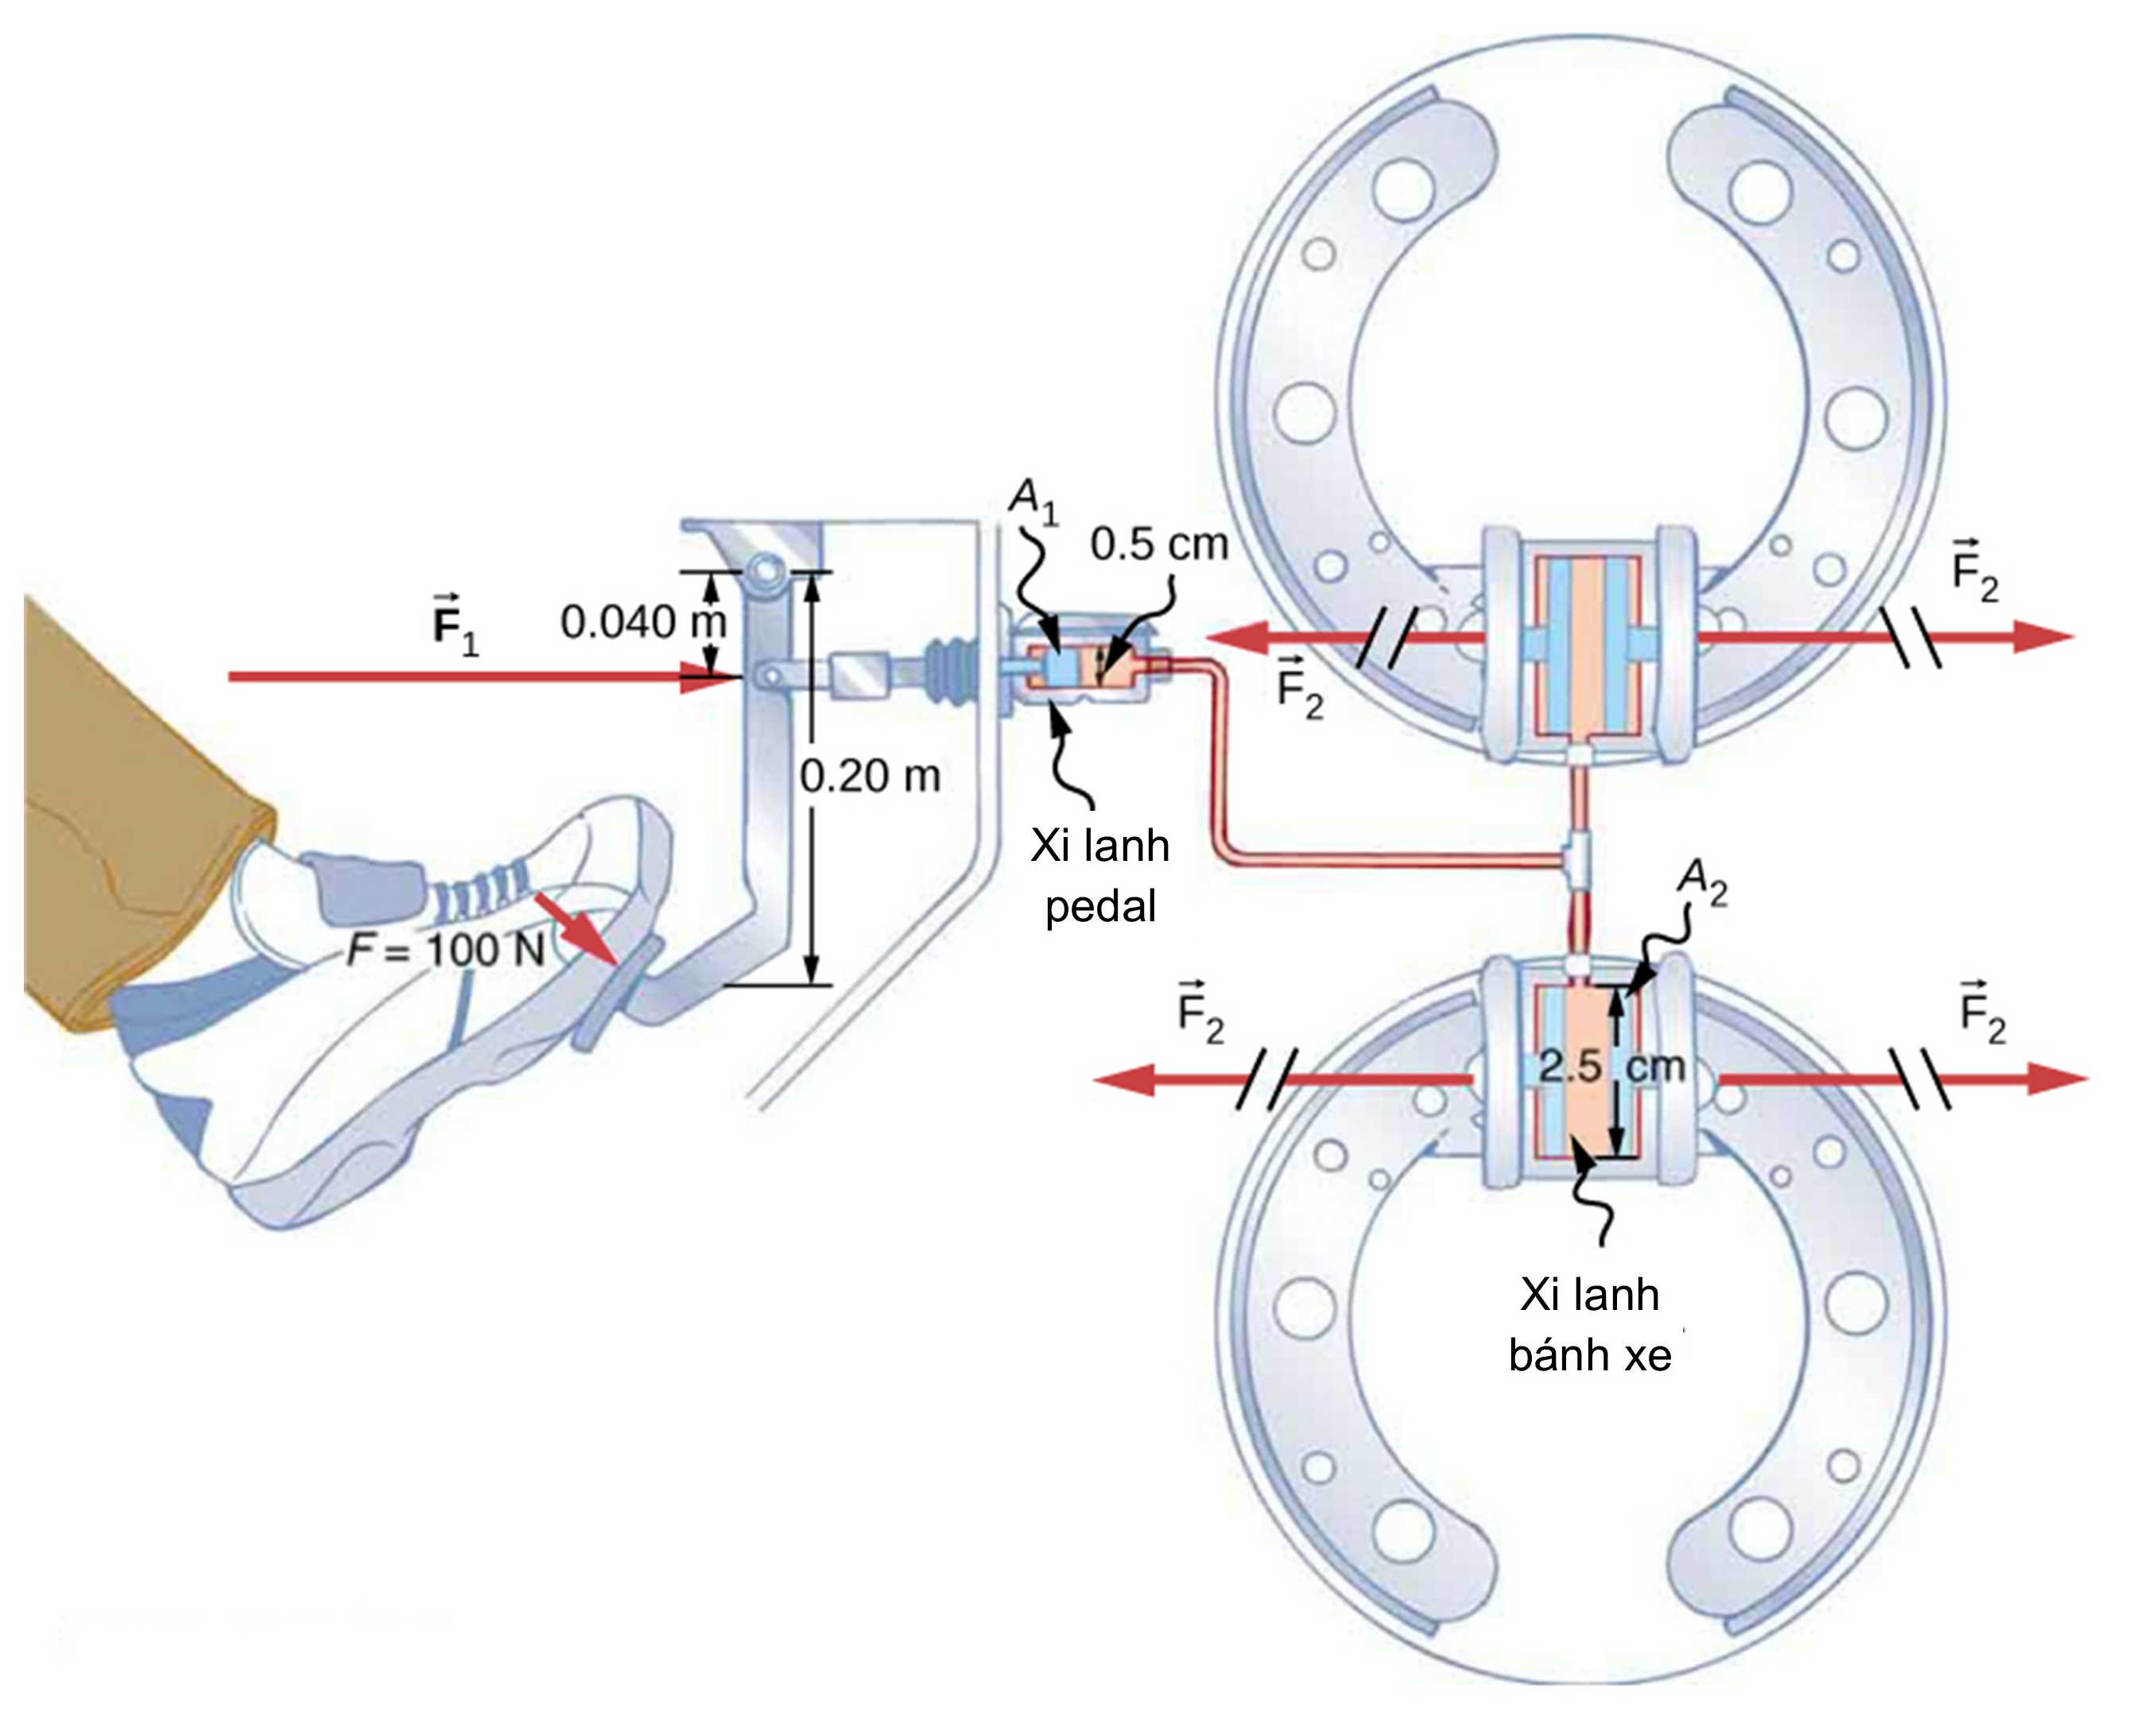
\includegraphics[width= 1\linewidth]{23}
		\caption{\small\textit{\color{timhieukhoahoc}Hình $12$. Hệ thống phanh xe sử dụng thủy lực.}}
		\vspace*{-10pt}
	\end{figure}
	Một ví dụ thú vị khác là trong hệ thống phanh xe sử dụng thủy lực (Hình $12$). Khi người lái xe ấn vào chân phanh, cần phanh thực chất có cấu tạo là một đòn bẩy nên lực nhấn vào hệ thống phanh sẽ lớn hơn nhiều lực đạp do tay đòn của nó ngắn hơn (ví dụ $4$ cm so với $20$ cm như trong hình). Lực nhấn này tác động vào một xi lanh có đường kính nhỏ ($0,5$ cm trong hình). Nhờ hệ thống thủy lực, lực tác động lên má phanh lại được khuyếch đại một lần nữa (bạn đọc có thể tự tính xem lực đạp $100N$ ban đầu của người lái xe được khuyếch đại thành lực có độ lớn bao nhiêu tại má phanh). Một điều đáng chú ý khác là hệ thống thủy lực cũng có thể phanh nhiều bánh xe cùng lúc, với mỗi bánh xe ta chỉ cần trang bị thêm một xi lanh nối vào hệ thống thủy lực. Tuy nhiên, như nguyên tắc trong tất cả các hệ thống thủy lực khác, khi ta được lợi về lực thì sẽ thiệt về quãng đường. Vì công do người thực hiện và công tác động lên các bánh xe là như nhau nên với cùng một khoảng cách đạp chân quãng đường di chuyển của xi lanh ở mỗi bánh xe sẽ càng ngắn nếu ta có càng nhiều bánh xe. 
	\vskip 0.1cm
	Với những phương tiện có quán tính lớn, ví dụ xe ủi, người ta có thể lắp đặt thêm hệ thống sử dụng chân không hoặc sử dụng phanh có động cơ thay vì đạp chân một cách thủ công. Trong các máy bay, hệ thống thủy lực không chỉ được dùng cho hệ thống phanh mà còn có nhiều tác dụng khác. Với sự kết hợp các bồn chứa chất lỏng, van định hướng và nhiều piston, người ta có thể điều chỉnh các bộ phận phức tạp của máy bay như cánh, đuôi, bộ phận hạ cánh, ...
	\begin{figure}[H]
		\vspace*{-5pt}
		\centering
		\captionsetup{labelformat= empty, justification=centering}
		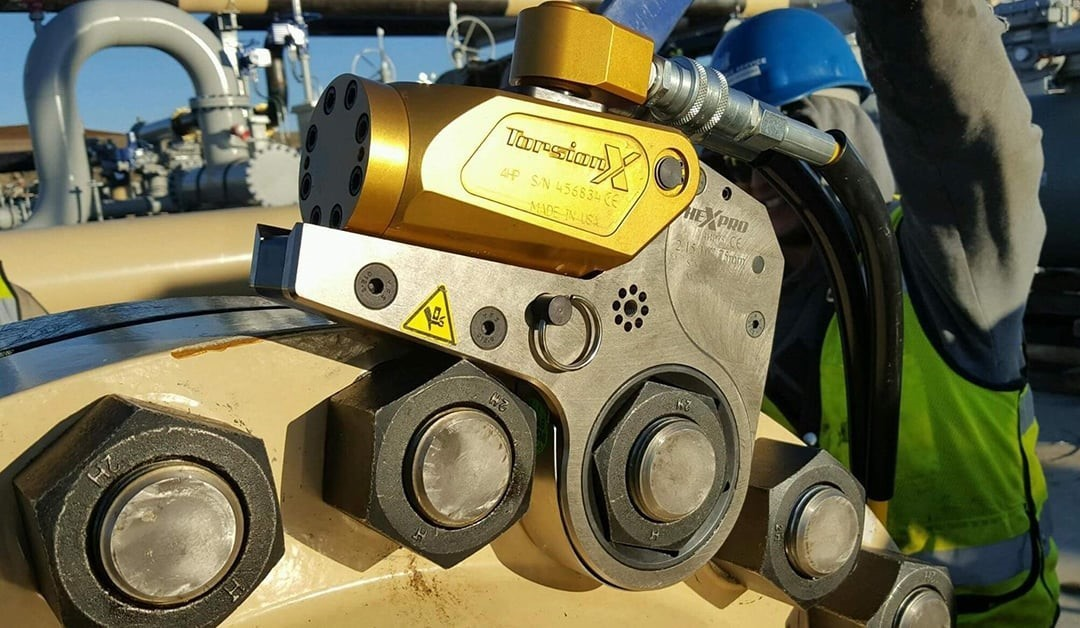
\includegraphics[width= 1\linewidth]{24}
		
		\vspace*{4pt}
		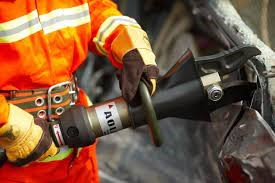
\includegraphics[width= 1\linewidth]{25}
		\caption{\small\textit{\color{timhieukhoahoc}Hình $13$. Một số công cụ lao động thủy lực. Trên: cờ lê thủy lực. Dưới: máy cắt thủy lực}}
		\vspace*{-10pt}
	\end{figure}
	Hệ thống thủy lực cũng được sử dụng cho các công cụ cầm tay, ví dụ như cờ lê thủy lực, máy cắt thủy lực, ... 
	\vskip 0.1cm
	$\pmb{3.}$ \textbf{\color{timhieukhoahoc}Đôi nét về lịch sử: Joseph Bramah và William Armstrong}
	\begin{figure}[H]
		\vspace*{-5pt}
		\centering
		\captionsetup{labelformat= empty, justification=centering}
		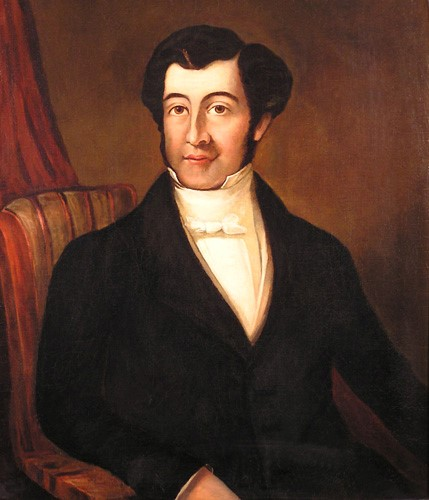
\includegraphics[width= 1\linewidth]{26}
		\caption{\small\textit{\color{timhieukhoahoc}Joseph Bramah $(1748-1814)$.}}
		\vspace*{-10pt}
	\end{figure}
	Về mặt lịch sử, tuy rằng Pascal đã trình bày lý thuyết về cách khuyếch đại lực sử dụng thủy lực từ thế kỷ $17$, các thiết bị sử dụng nguyên lý này chỉ xuất hiện lần đầu trong thực tiễn vào cuối thế kỷ $18$ với  máy ép thủy lực đầu tiên được Joseph Bramah chế tạo. Sự kiện này đánh dấu một bước tiến quan trọng của cuộc cách mạng công nghiệp ở nước Anh khi đó. Nhiều cỗ máy thủy lực tiếp theo đã được sáng chế phục vụ các công việc khác nhau trong sản xuất. Đến giữa thế kỷ $19$, William Armstrong đã nghiên cứu cách sử dụng thủy lực cho các cần cẩu cỡ lớn phục vụ vận chuyển hàng hóa ở các bến cảng và bắt đầu tiến hành sản xuất chúng hàng loạt với nhà máy có quy mô lên đến $20000$ công nhân. Cây cầu ở thành phố Newcastle cũng được Armstrong xây dựng lại với hệ thống thủy lực cho phép nâng nhịp cầu lên khi các tàu thuyền lớn cần đi qua để vào cảng.
	\vskip 0.1cm
	Dựa trên ý tưởng trước đó của Bramah, Armstrong tiến hành thử nghiệm các hệ thống cung cấp áp lực cho hoạt động của các máy thủy lực. Sau thử nghiệm thất bại với tháp nước do chiều cao cần xây dựng quá lớn, ông sử dụng hệ thống gồm bình chứa lớn với một piston đè lên khối nước bên dưới. Phía trên piston có nhiều quả nặng khối lượng lớn tạo áp suất lên khối nước. Đáy bình được nối với hệ thống đường ống dẫn đến nơi các hệ thống máy móc cần hoạt động, tương tự như mạng điện của chúng ta ngày nay. Những bình chứa của Armstrong còn được gọi là các thiết bị tích tụ thủy lực. Chúng nhanh chóng được phổ biến ở nước Anh cũng như một số nơi khác ở châu Âu. Các mạng áp suất thủy lực này vẫn được duy trì hoạt động cho đến những năm $70$ của thế kỷ $20$. Nhiều thiết bị tích tụ thủy lực hiện đại dạng cải tiến dùng khí nén hoặc lò xo được sử dụng trong nhiều máy móc công nghiệp đa dạng ngày nay.
	\begin{figure}[H]
		\vspace*{-5pt}
		\centering
		\captionsetup{labelformat= empty, justification=centering}
		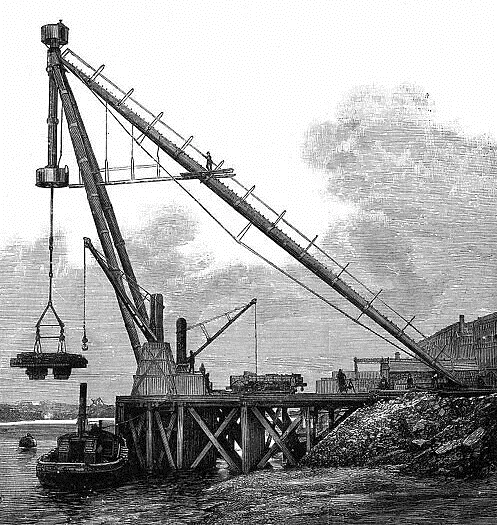
\includegraphics[width= 1\linewidth]{28}
		\caption{\small\textit{\color{timhieukhoahoc}Cần cẩu thủy lực của Armstrong có thể nâng các khối hàng hóa nặng hàng trăm tấn.}}
		\vspace*{-10pt}
	\end{figure}
	Đặc biệt, Armstrong đã tiên đoán từ thế kỷ $19$ rằng các nhiên liệu như than đá sẽ cần được thay thế bằng các nguồn năng lượng như thủy điện hay năng lượng mặt trời. Ngôi nhà của Armstrong ở Newcastle cũng là ngôi nhà đầu tiên trên thế giới được thắp sáng nhờ thủy điện.
	\begin{figure}[H]
		\vspace*{-5pt}
		\centering
		\captionsetup{labelformat= empty, justification=centering}
		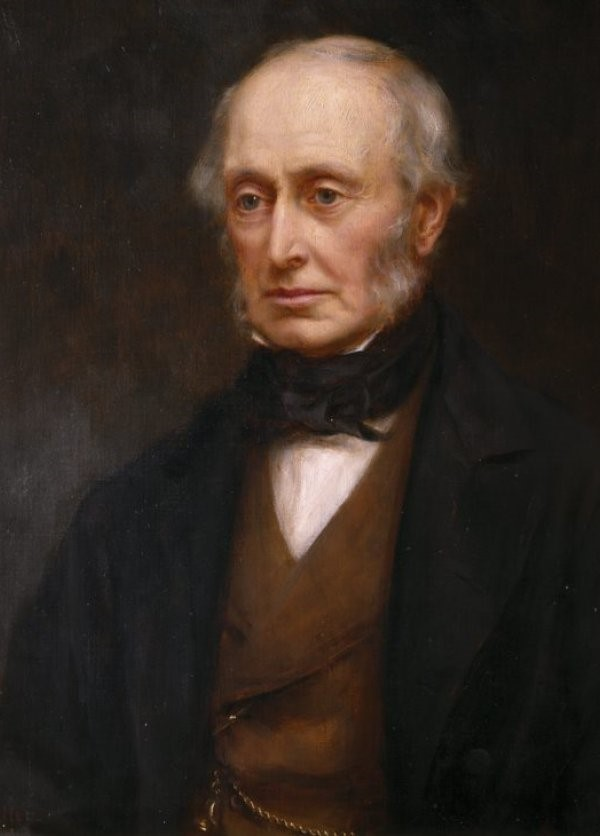
\includegraphics[width= 1\linewidth]{27}
		\caption{\small\textit{\color{timhieukhoahoc}William Armstrong $(1810 - 1900)$.}}
		\vspace*{-10pt}
	\end{figure}
	$\pmb{4.}$ \textbf{\color{timhieukhoahoc}Kết luận}
	\vskip 0.1cm
	Bản thân Pascal cũng nhận định rằng một bình chứa nước có thể trở thành một loại máy cơ học mới cho phép khuyếch đại lực đến bất cứ mức độ nào. Tuy nhiên, chắc ông cũng sẽ không khỏi ngạc nhiên với những ứng dụng đa dạng của các hệ thống thủy lực ngày nay. Các hiện tượng về chất lỏng cũng như chất khí còn rất nhiều điều thú vị mà Pi sẽ giới thiệu với bạn đọc trong các số sau này.
	\vskip 0.1cm
	\textbf{\color{timhieukhoahoc}Tài liệu tham khảo}
	\vskip 0.1cm
	Hughes, S., \& Gurung, S. ($2014$). Exploring the boundary between a siphon and barometer in a hypobaric chamber. \textit{Scientific Reports}, $4(1)$. \url{https://doi.org/10.1038/srep04741}
\end{multicols}


